\chapter{Approach}\label{chap:approach}

In the field of unsupervised instance detection and segmentation, CutLER~\cite{wang2023cut} gives a strong performance by exploiting a  object-centric prior by training on ImageNet~\cite{deng2009imagenet}, as most images contain a single
object in the center of the frame.  Due to its strong instance discrimination abilities, CutLER is the current state-of-the-art method for this task.

In this chapter, we are exploring the limitation of CutLER, looking deeper into the special cases where CutLER fails such as overlapping instances and complex backgrounds. We also analyze the change in performance when the model is trained without overlapping instances, as a main reason for CutLER's superior  performance is it's object-centric prior~\cite{engstler2023understanding}. Using the gathered information from the analysis, we introduce a hypothesis to refine Maskcut masks using CutLER outputs to train the model from scratch to obtain a better evaluation score across a variety of datasets.

\section{Limitations of CutLER}
Even though CutLER is the state-of-the-art model for unsupervised instance detection and segmentation, it still has several drawbacks. We go through some of them in this section.

\subsection{Overlapping Instances}
\begin{figure*}
	\centering
	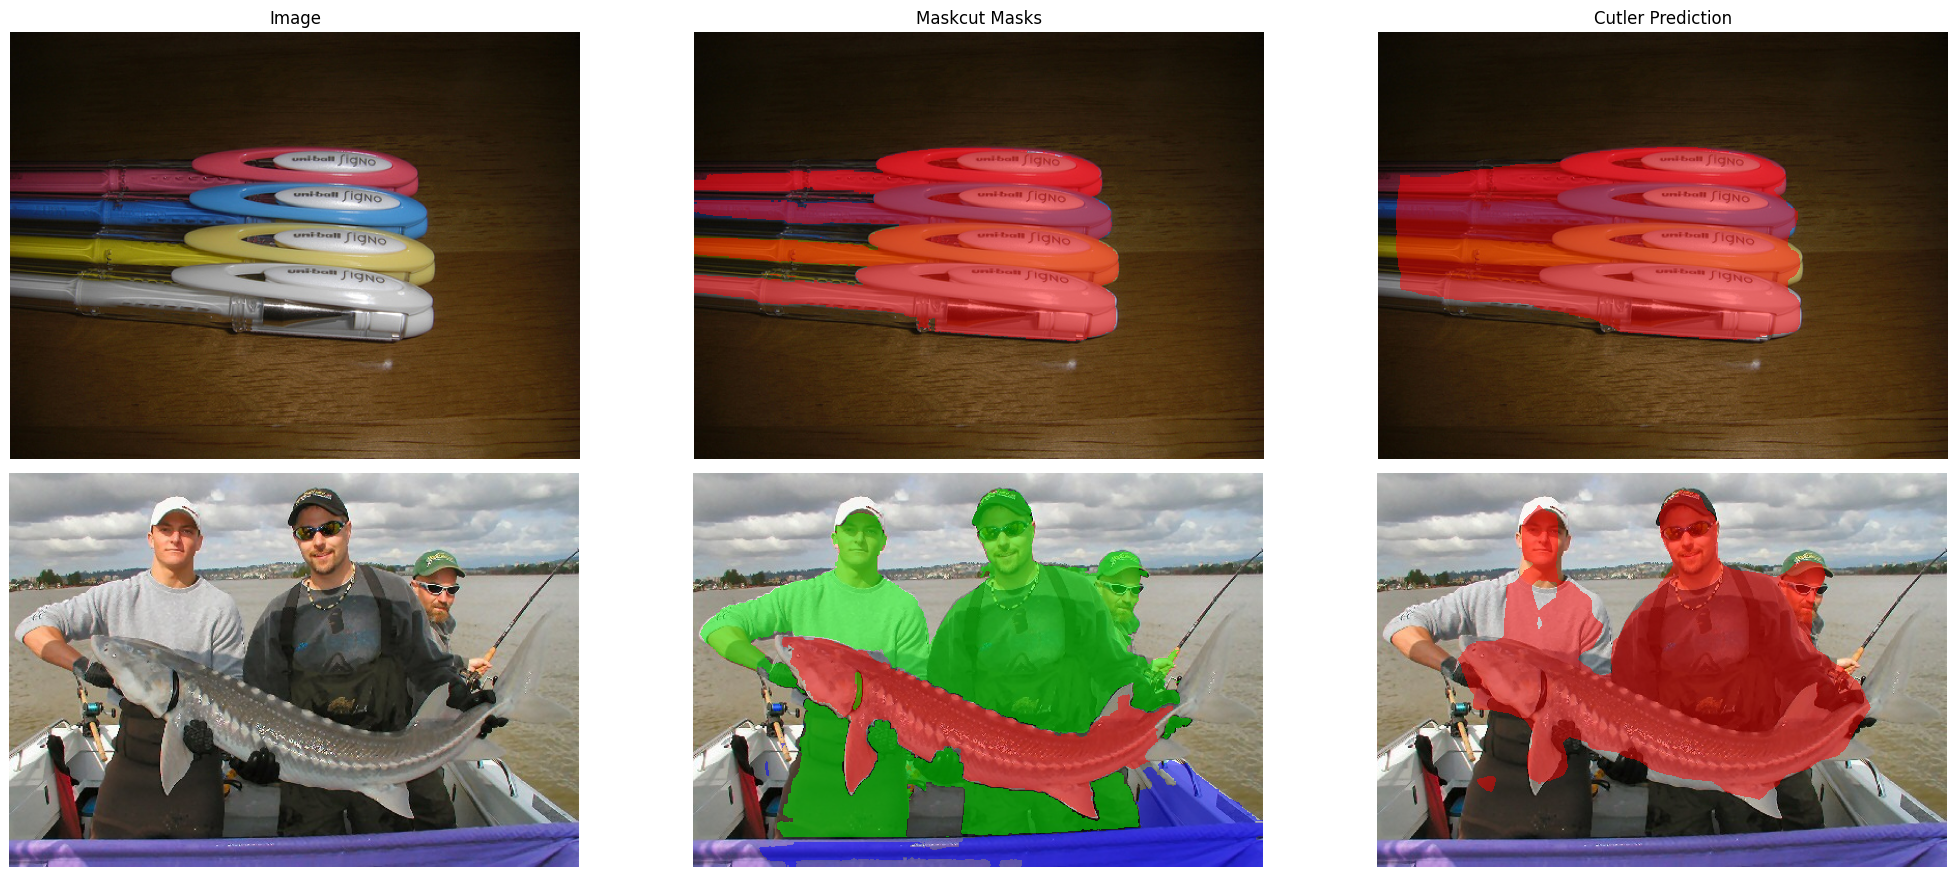
\includegraphics[width=1\textwidth]{Images/main/cutler-prob-overlap.png}
	\caption[\textbf{Cutler's Performance on Images with Overlapping Instances}]{\textbf{Grouping of overlapping instances} in MaskCut and CutLER outputs, which is a common problem in most of the existing unsupervised instance detection methods.}
	\label{fig:cutler_overlapping_instances_eg}
\end{figure*}

Identifying instances using an unsupervised instance detection or segmentation method presents significant challenges, especially when instances are closely positioned or overlapping in an image. In such scenarios, the algorithm must discern subtle differences in texture, color, and shape without the benefit of labeled training data. Overlapping objects often blend together, making it difficult for the model to accurately segment and differentiate them as distinct entities. This lack of explicit supervision complicates the model's ability to learn and generalize the spatial relationships and boundaries between objects. Moreover, unsupervised methods typically rely on clustering and feature extraction techniques, which may not be robust enough to handle the complexities of overlapping instances, leading to errors in segmentation and misidentification.

As illustrated in Fig.~\ref{fig:cutler_overlapping_instances_eg}, in almost all cases of images with overlapping instances, MaskCut and CutLER groups those instances together. As a result, in images with instance overlap, unsupervised methods gives semantic segmentation like outputs instead of instance segmentation.

The problem is not exclusive to CutLER, but most of the existing methods~\cite{engstler2023understanding, cond1_support_2, Wang_2022_CVPR} also address this issue. Solving this problem requires, for instance, the learning of an instance-variant representation, which is a challenging task. 

Another solution to address the grouping of instances would be to provide explicit semantic information of instances during training. It is explored in Wang et al. (2023)~\cite{wang2023cut} by testing with low-shot settings, ie, 2\% and 5\% labeled data, CutLER achieves 5.4\% and 7.3\% higher \(AP_{box}\) than the fully supervised MoCo-v2 with better separation of close and overlapping instances. But as our approach focuses solely on improving the unsupervised instance detection performance, the problem of grouping instances remains unsolved in our approach as well. But we intent to explore the influence of overlapping instances on CutLER training and evaluation which is explained in detail in section~\ref{section:analysis_ol_instancs}.

\subsection{Images with Complex Background}
\begin{figure*}
	\centering
	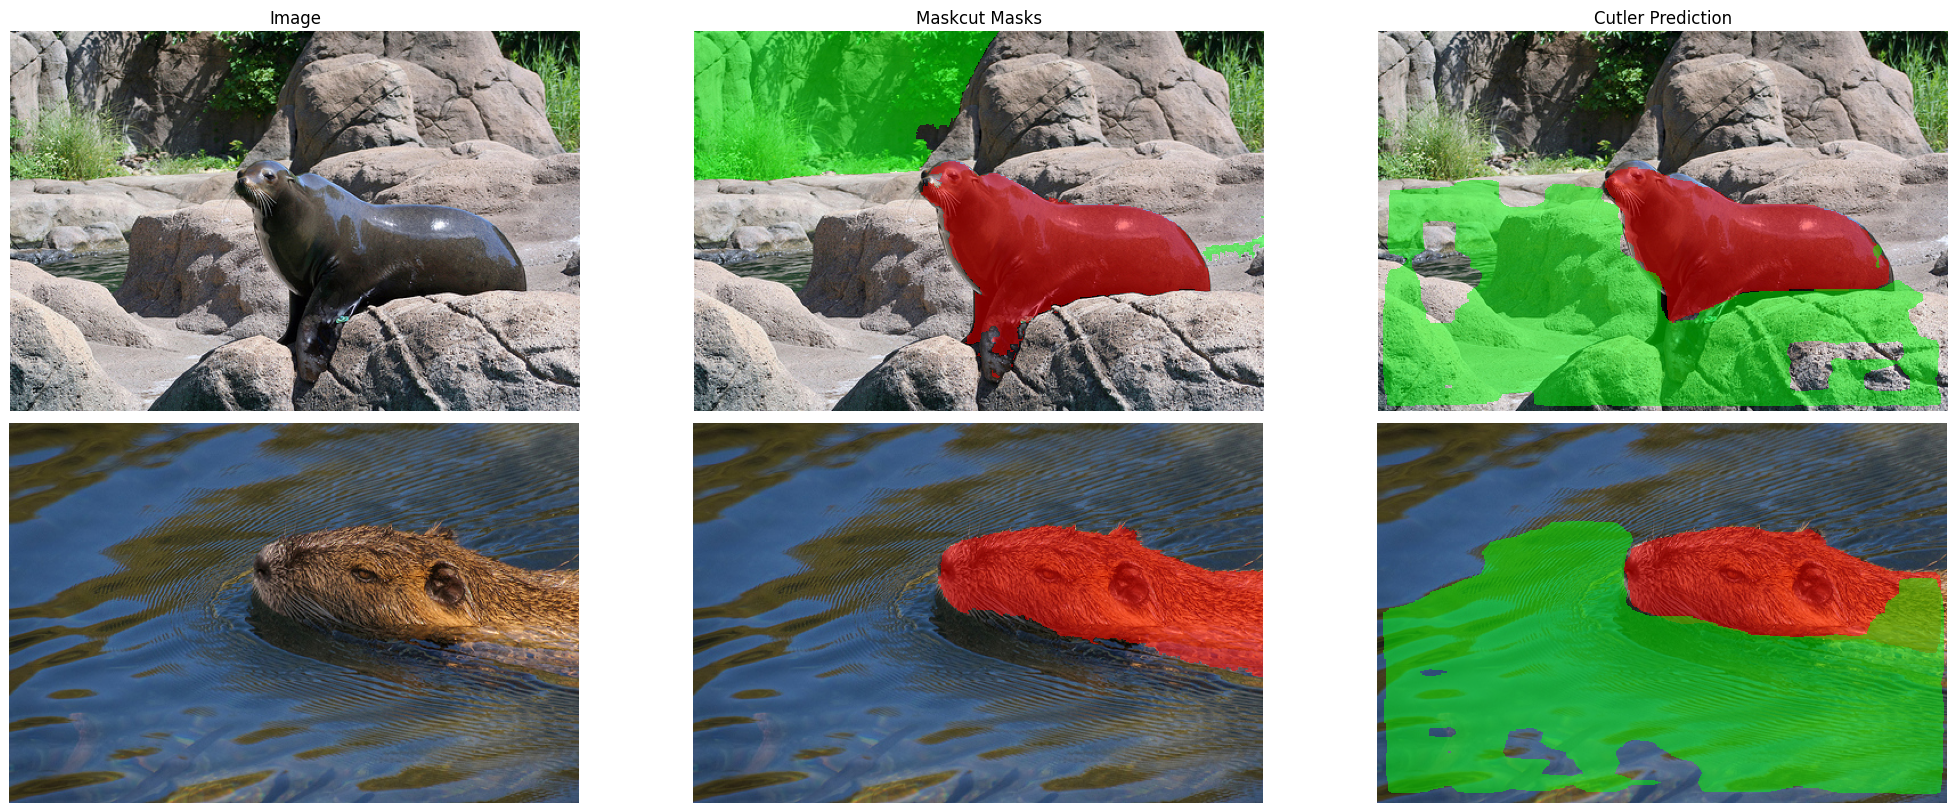
\includegraphics[width=1\textwidth]{Images/main/cutler-prob-noisy-bg.png}
	\caption[\textbf{Cutler's Performance on Images with Complex Background}]{\textbf{Images with complex backgrounds} impacting MaskCut and CutLER outputs, leading to undesired background mask generation}
	\label{fig:cutler_noisy_bg_eg}
\end{figure*}

The quality pseudo-ground truths generated by MaskCut can significantly affect the performance of CutLER. These pseudo-ground truths often contain inaccuracies due to imperfect initial segmentation, which can arise from factors like complex backgrounds, occlusions, and variations in object appearance. Such imperfections can mislead the model, causing it to learn incorrect features and boundaries, ultimately degrading the quality of instance detection and segmentation. The presence of incorrect masks can lead to overfitting on incorrect patterns or failure to generalize properly across different instances. To mitigate these issues, techniques like iterative refinement, robust loss functions, and the incorporation of consistency constraints have been proposed. Tang et al.~\cite{Tang_2018_CVPR} and Wang et al.~\cite{ziegler2022selfsupervisedlearningobjectparts} explore these approaches, highlighting the importance of addressing inaccuracies in pseudo-ground truths to enhance the robustness of unsupervised instance detection and segmentation methods.

In our approach, we intent to address the issue of unwanted masks generated due to complex backgrounds as shown in Fig.~\ref{fig:cutler_noisy_bg_eg}. Such masks can not only be present in the MaskCut masks which act as the pseudo-ground truth for CutLER training, but also in the CutLER predictions itself. As per our observation, the mask filtration strategy used by the baseline doesn't address this issue, which is explained in detail in section~\ref{sec:baseline_mask_filteration}.

In CutLER, a self-training loop is implemented to iteratively refine the pseudo ground truth masks. We hypothesis that removing undesired background mask before training and self-training phases could improve the performance of the model. We intent to implement this hypothesis by modifying the mask filtration algorithm used to refine pseudo-ground truth masks before each self-training loop in the baseline method.
\begin{figure*}
	\centering
	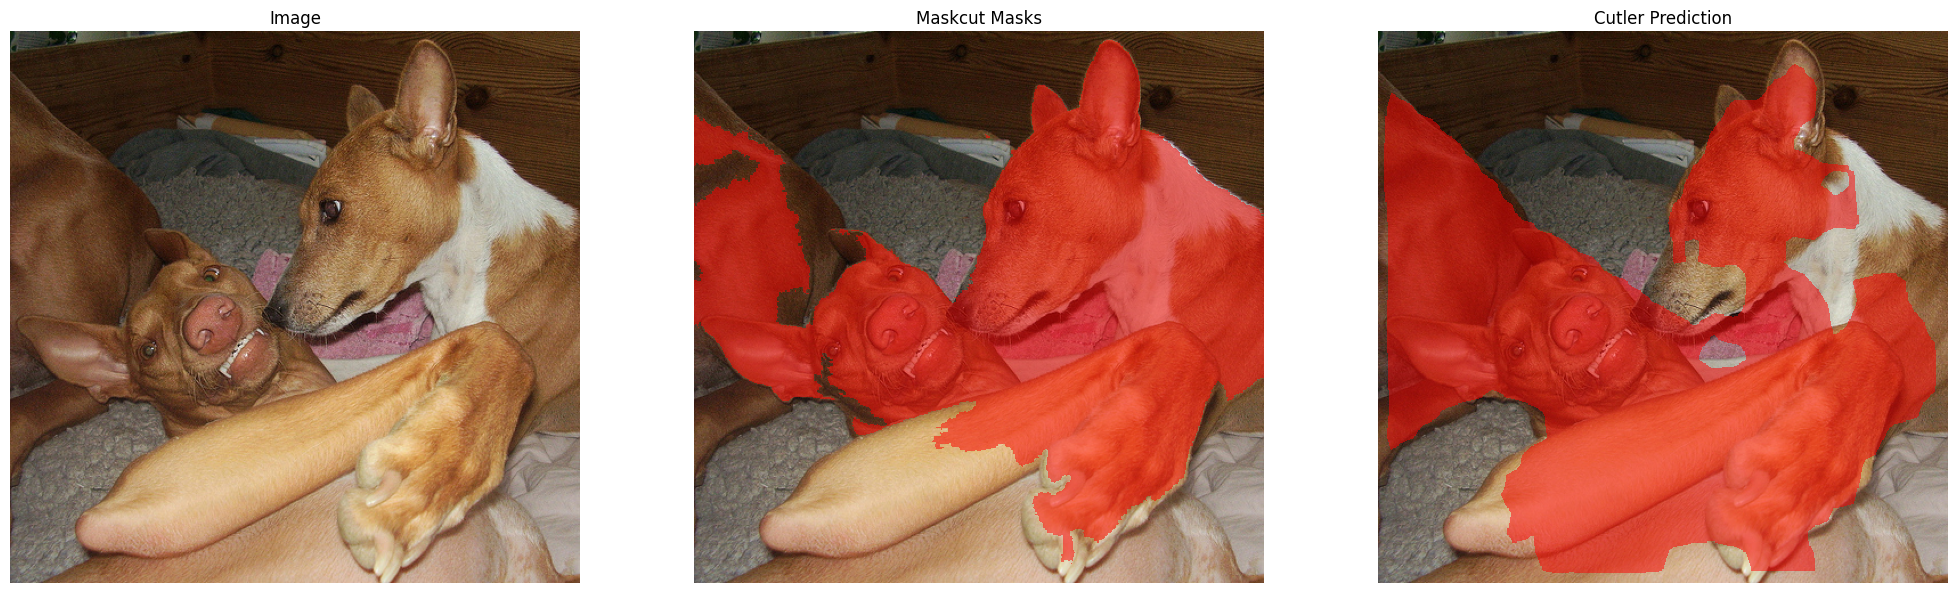
\includegraphics[width=1\textwidth]{Images/main/cutler_problem_3.png}
	\caption[\textbf{Dependence on Initial Masks}]{\textbf{Dependence on initial masks} reflected on the final CutLER prediction}
	\label{fig:intial_mask_dependence}
\end{figure*}
\subsection{Dependence on Initial Masks}

CutLER relies on initial masks provided by MaskCut. If these initial masks are of poor quality, the performance of CutLER may be adversely affected. As MaskCut produces the masks based on a hyperparameter N (maximum number of masks generated per image), pseudo-ground truth can have incomplete masks or grouped instances.

In challenging scenarios with cluttered backgrounds, occlusions or low-quality images, MaskCut could produce noisy masks as in Fig.~\ref{fig:intial_mask_dependence} which can also affect the quality of CutLER predictions. One common method to filter out good masks is thresholding, which is used in the baseline and our approach during self-training.

To address this issue before self training, in our approach, we filter the MaskCut masks using the CutLER predictions and train from scratch, assuming the learning from scratch using better quality masks could improve the performance of the model. The approach is explained in detail in section~\ref{section:proposed_method}.

\section{Impact of Overlapping Instances}
\label{section:analysis_ol_instancs}
When instances are closely positioned or overlapping in an image, it often makes the model difficult to accurately segment and differentiate them as distinct entities without supervised semantic input \cite{kara2022image}. But based on the hypothesis that CutLER benefits from it's object-centric prior from training on Imagenet~\cite{engstler2023understanding}, we hypothesis that CutLER when trained with images without overlapping instances of ImageNet might perform better than the model trained with all images. It also intent to investigate whether a model trained without any overlapping instances would help to detect individual instances better in images with overlapping instances.

For the sake of completeness and to observe whether there is any relative improvement or loss, we compare three approaches of training CutLER. 1) Using all images of ImageNet (Same as the baseline). 2) Using images without any overlapping instances, 3)  Only using images with overlapping instances. We expect that the model trained without overlapping instances will outperform the baseline, while the model trained exclusively on images with overlapping instances will likely underperform compared to the baseline. Splitting the evaluation dataset according to these three approaches should also reveal a similar performance pattern. Our hypotheses is supported by the positive results from the experiments in section <SECNO>.

To test the hypothesis, we make use of ground truth bounding box annotations provided by ImageNet and the images with an overlap(IoU) of \(\tau > \text{10\%}\) is taken as the criteria to filter images for approach 2 and 3. As ImageNet contains mostly object-centric single instance images, 3rd approach (only using images with overlapping instances) would have significantly less number of training images compared to the other two approaches. Specifically, Approach 3 utilizes 6\% of the annotated ImageNet dataset, while Approach 2 uses the remaining 94\%. Given the significantly smaller training sample size in Approach 3, a fair comparison isn't possible. Therefore, we focus on Approach 2 for comparison with the baseline.

Through this approach, we expect to observe an improvement by using less training data. But using this method in unsupervised fashion is rather difficult. Due to the grouping of nearby instances, the process of filtering images with overlapping instance is extremely challenging. Hence these tests are carried out using bounding box annotations. Nevertheless, the approach gives insights on the influence of overlapping instances in training that can be useful for future research.

\section{Mask Filtering}
\begin{figure*}
	\centering
	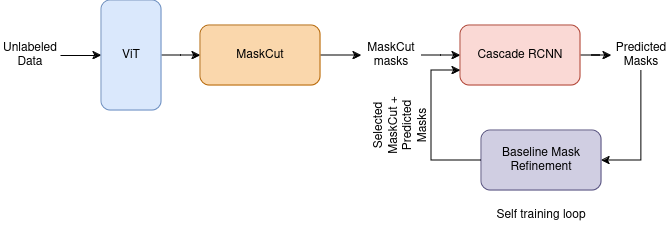
\includegraphics[width=1\textwidth]{Images/main/baseline_method.png}
	\caption[\textbf{Baseline Training Pipeline}]{\textbf{Baseline training pipeline} with repeated mask filtration and self-training}
	\label{fig:baseline_training}
\end{figure*}
Generating initial pseudo-ground truth masks using a pre-trained model or some heuristic methods may contain errors or inaccuracies. Hence, iteratively refining the pseudo-ground truth masks(self-training) is essential for improving the performance of the model. Iterative refinement helps in progressively reducing this noise, leading to cleaner and more reliable labels~\cite{xie2020selftrainingnoisystudentimproves}. Popular refinement methods incorporate strategies like thresholding, where only high-confidence predictions are used for retraining, or use ensemble methods to combine predictions from multiple models for more reliable masks.

\subsection{Baseline Mask Filtering Method}
\label{sec:baseline_mask_filteration}

In CutLER, thesholding method is used to combine prediction masks and pseudo-ground truth masks to create more reliable masks for the next self-training round. As illustrated in Fig.~\ref{fig:baseline_training}, after the training for 160K iterations using MaskCut masks as pseudo-ground truth, masks are predicted for each image in ImageNet dataset (30 masks per image) using the trained model. Out of the 30 predicted masks, high-quality ones are filtered by applying a confidence score threshold of 0.7.

Batch IoU is calculated between the selected predicted masks and MaskCut masks. For mask pairs with an IoU below 0.5, the corresponding MaskCut masks are included, along with all selected predicted masks, to form the pseudo-ground truths for the next self-training stage. Intuitively, MaskCut masks that have less than 50\% overlap with the selected CutLER masks are also included alongside the CutLER masks. The goal is to retain as many non-overlapping masks as possible. However, always including masks that don't overlap with CutLER prediction masks may introduce irrelevant or unwanted masks into the pseudo-ground truth. This can affect the performance of the model. Our approach addresses the issue in section~\ref{section:proposed_method}.

For further self-training loops, the same procedure repeats, except that instead of MaskCut masks, pseudo-ground truth masks of the last round are used to compare with the predicted CutLER masks. Performance of the model claims to have improved upto 3 self-training loops by the authors. We will be running 2 self-training loops for both the baseline and proposed method. The only difference in the self training loop in our approach is the mask filtration method.

\subsection{Proposed Mask Filtering Method}
\label{section:proposed_method}

\begin{figure*}
	\centering
	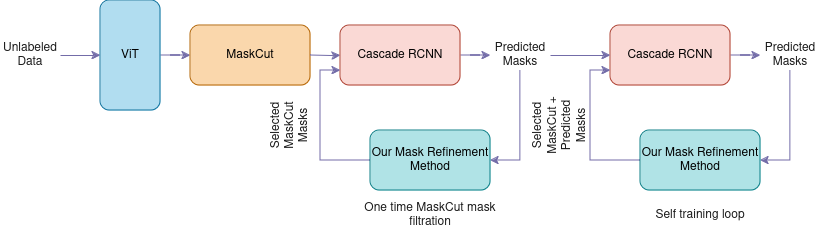
\includegraphics[width=1\textwidth]{Images/main/proposed_method.png}
	\caption[\textbf{Proposed Training Pipeline}]{\textbf{Proposed training pipeline} featuring a one-time MaskCut mask filtration followed by multiple self-training loops with our mask filtration method.}
	\label{fig:proposed_training}
\end{figure*}
Emphasizing quality over quantity, we introduce an improved approach for mask filtration. Noting that the current mask filtration method in CutLER tends to include unwanted background masks in its pseudo ground truths, we propose to enhance the process by removing ambiguous masks from the ground truth instead of retaining them. This adjustment aims to improve the overall quality and reliability of the pseudo ground truths, leading to better model performance.

\begin{figure*}
	\centering
	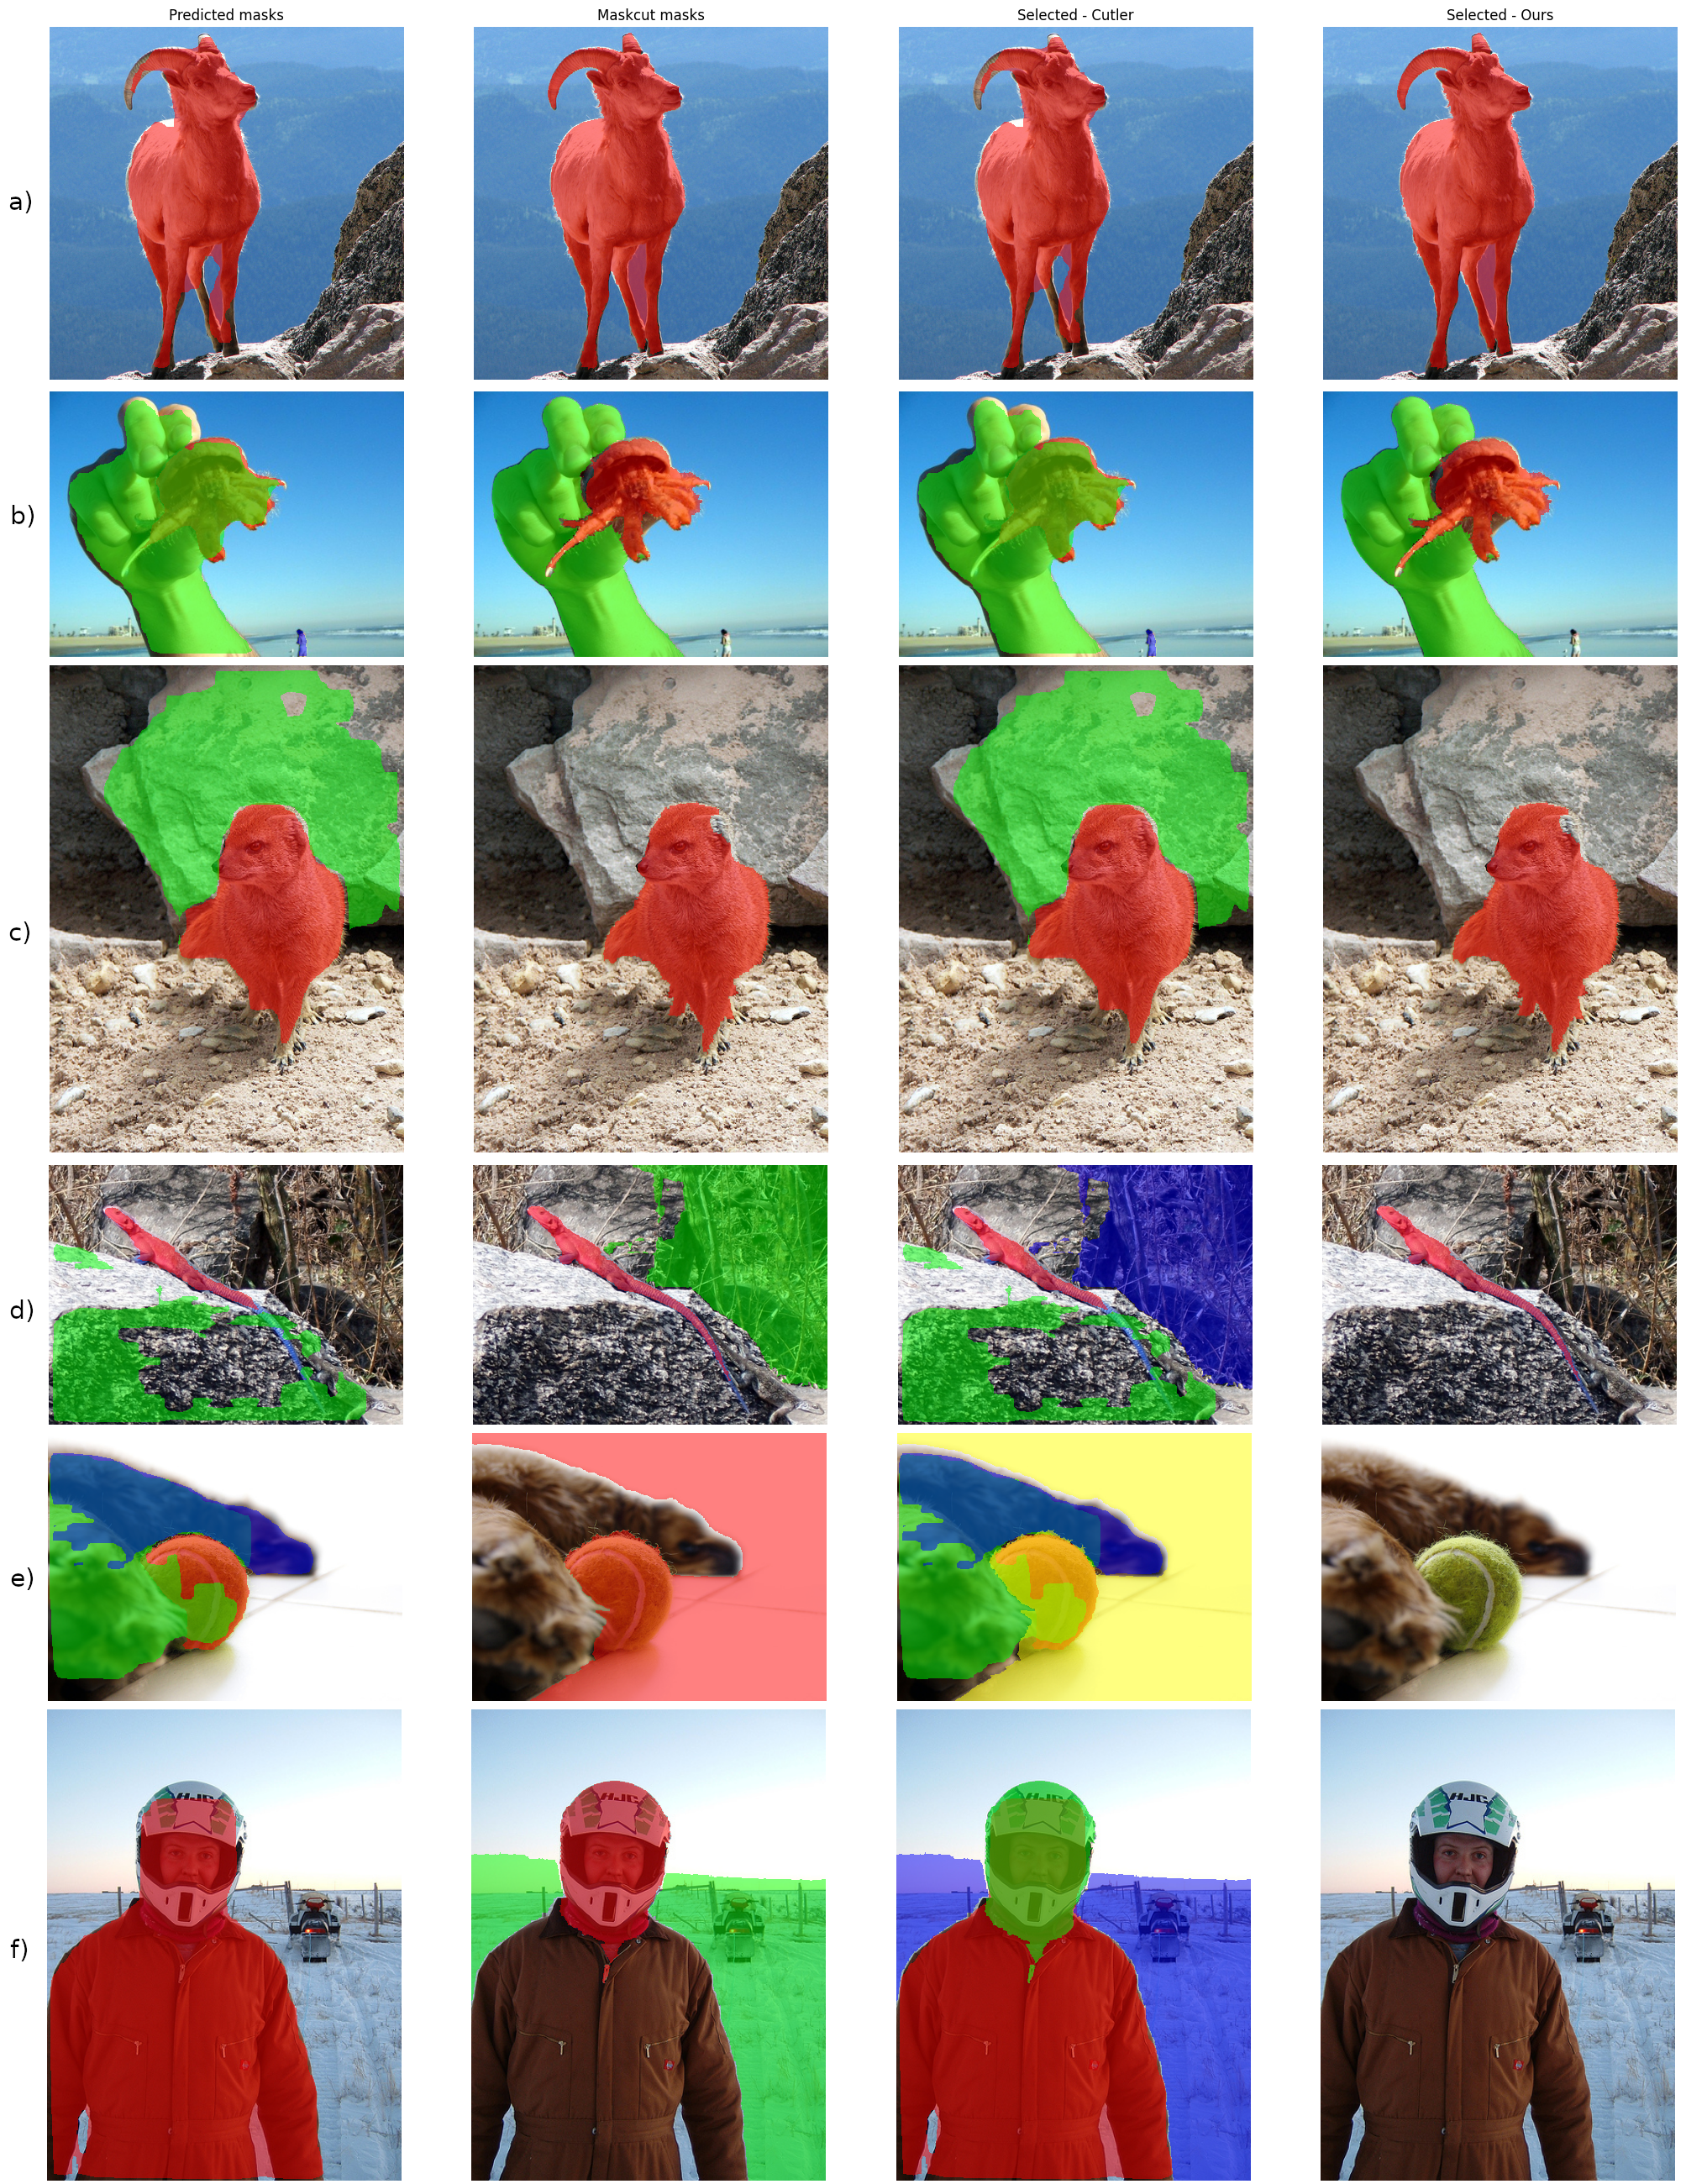
\includegraphics[width=1\textwidth]{Images/main/filtered_mask_comparison.png}
	\caption[\textbf{Mask Filtration Outputs - Baseline vs Ours}]{\textbf{Comparison of filtered masks} produced by the baseline and our method. Examples illustrates Cutler prediction masks, MaskCut masks, masks selected by Cutler and masks selected by our method respectively (left to right)}
	\label{fig:filtered_mask_comparison}
\end{figure*}
As illustrated in Fig.~\ref{fig:proposed_training}, we introduce an extra step to refine MaskCut masks by preserving the masks with high certainty by comparing with CutLER predictions. After the first training phase, like in the baseline, high-quality predicted masks are filtered by applying a confidence score threshold of 0.7. Instead of creating the new pseudo-ground truth by selecting masks from both MaskCut masks and CutLER prediction masks, we focus solely on filtering MaskCut masks. Rather than selecting MaskCut masks corresponding to mask pairs with an IoU < 0.5 from the batch IoU matrix, we choose MaskCut masks that correspond to mask pairs with an IoU > 0.5. This selected MaskCut masks are treated as the new pseudo-ground truth and we train from scratch for 160K iterations. With the filtered high quality masks in hand, we expect to achieve a better performance. It’s important to note that if no masks are selected for an image, that image is removed from the training set, resulting in a smaller dataset and reducing the training time (Around 130K images are dropped from ImageNet during this stage). This approach effectively eliminates potentially unwanted masks from the pseudo-ground truth, ensuring higher quality and more accurate mask predictions. For self-training, we follow training pipeline of the baseline, training 80K iterations are without using DropLoss.

Figure~\ref{fig:filtered_mask_comparison} illustrates the differences between the masks selected by our method and the baseline method across few example images. For most images with single instances with distinguishable background, there is no significant difference between masks selected by baseline and our method as given in Fig.~\ref{fig:filtered_mask_comparison}~(a). Unfortunately a huge part of ImageNet dataset contains single instance object-centric images with simple backgrounds. Hence the improvement that we might obtain can be minimal. Nevertheless, our method works best for examples shown in Fig.~\ref{fig:filtered_mask_comparison}~(b-d). In Fig.~\ref{fig:filtered_mask_comparison}~(b-c) our approach successfully removes incorrect masks introduced by CutLER that are overlaid on better MaskCut masks. In Fig.~\ref{fig:filtered_mask_comparison}~(d), despite both MaskCut and CutLER containing noisy masks, our method effectively filters out these imperfections.

As we discussed earlier in this section, some images are dropped from the training dataset for not having any selected masks. In Fig.~\ref{fig:filtered_mask_comparison}~(e), the image is dropped due to no selected masks, but CutLER prediction and mask selection are also bad. But in Fig.~\ref{fig:filtered_mask_comparison}~(f) CutLER selection is certainly better compared to predicted masks. But the image will be dropped in our method. These examples reaffirms that we compromise on quantity for quality in our approach. But nevertheless our method outperforms baseline even with lesser data.

Even though the method might improve the precision, as we are limiting the range of exploration by removing more masks, we expect the recall to decrease by a small factor. However, our experiments indicate that this change is negligibly small. Detailed results and analysis can be found in the Experiments section.

%\begin{figure*}[h]
%	\centering
%	\begin{subfigure}[b]{0.47\textwidth}
%		\centering
%		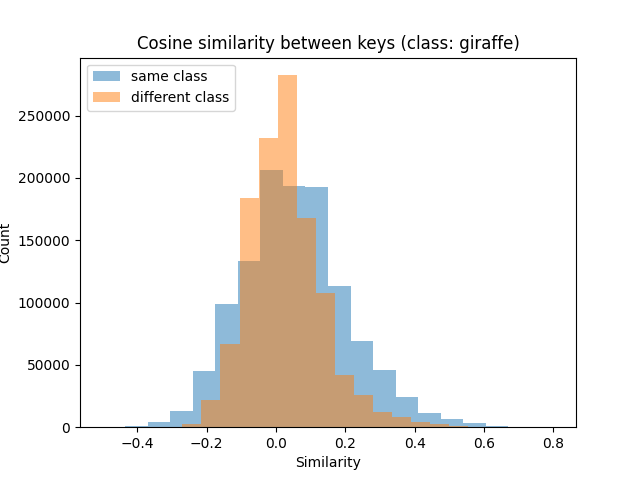
\includegraphics[width=\textwidth]{Images/same_vs_diff_class/plot_giraffe_cosine.png}
%		\caption{Cosine similarity}
%	\end{subfigure}
%	\quad
%	\begin{subfigure}[b]{0.47\textwidth}  
%		\centering 
%		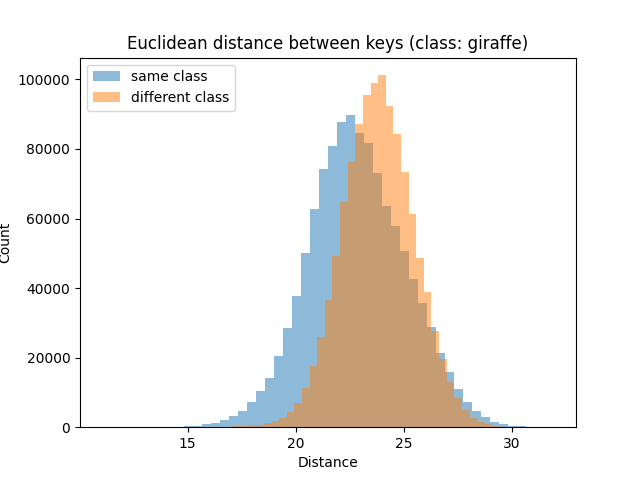
\includegraphics[width=\textwidth]{Images/same_vs_diff_class/plot_giraffe_euc.png}
%		\caption{Euclidean}
%	\end{subfigure}
%	\caption[\textbf{Comparison of keys of images of same and different classes}]{\textbf{Comparison of keys of images of same and different classes}. Shows the pattern of similarity scores and distance measure when comparing keys of same and different classes. Y axis shows number of images compared }
%	\label{fig:same_vs_diff}
%\end{figure*}